\documentclass[12pt,a4paper]{report}
\usepackage[utf8]{inputenc}
\usepackage{amsmath}
\usepackage{amsfonts}
\usepackage{amssymb}
\usepackage{graphicx}
\usepackage{enumitem}
\usepackage[left=2cm, right=2cm, top=4cm, bottom=2cm]{geometry}

\begin{document}
	\begin{titlepage}
		\centering
		{\scshape\LARGE Universidad Nacional Autónoma de México \par}
		\vspace{1cm}
		{\scshape\Large Probabilidad I\par}
		\vspace{1.5cm}
		{\huge\bfseries Tarea IV\par}
		\vspace{.5cm}

		{\Large\itshape Alan Ernesto Arteaga Vázquez \par}
		 \vspace{.5cm}
		{\Large\itshape Raúl Llamosas Alvarado \par}
		 \vspace{.5cm}
		{\Large\itshape Edgar Quiroz Castañeda \par}
	    \vspace{.5cm}
		{\Large\itshape Jean Paul Ruiz Melo\par}
		\vspace{.5cm}
		{\Large\itshape Sandra Del Mar Soto Corderi \par}

		\vfill
		 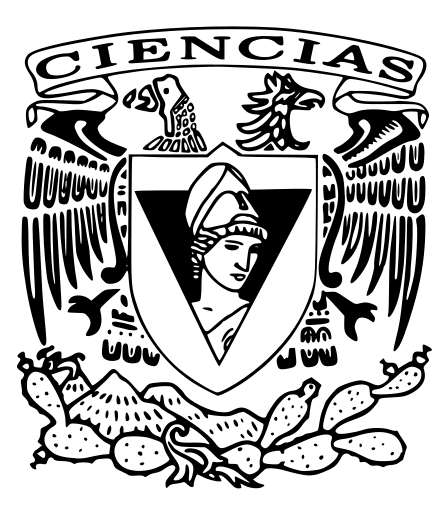
\includegraphics[width=0.5\textwidth]{escudo.png}
		\vfill

		{\large Lunes 15 de octubre del 2018 \par}
	\end{titlepage}

	\pagebreak
	\setlength{\voffset}{-0.75in}
	\setlength{\headsep}{5pt}

	\begin{enumerate}
		\item {
			Sea $A$ un evento $(A \in F)$. Definimos $X$ por
			\[
				X(\omega) =
				\begin{cases}
					1, $ si $\omega \in A\\
					0, $ si $\omega \not\in A
				\end{cases}
			\]
			¿Es $X$ variable aleatoria?
		}
		\item {
			Considere un espacio de probabilidad $\Omega = \{1, 2, 3, 4, 5, 6\}$ y
			$F = \{\emptyset, \Omega, \{2, 4, 6\}, \{1, 3, 4\}\}$.\\
			Sean $X_1, X_2 : \Omega \rightarrow \mathbb{R}$ definidas como
			\begin{align*}
				X_1(\omega) = \omega^2 & X_2(\omega) = \begin{cases}
																								1, \omega $ par$\\
																								0, \omega $ impar$
																							\end{cases}
			\end{align*}
			¿Son $X_1$ y $X_2$ variables aleatorias en este espacio de probabilidad?
		}
		\item {
			Sea $f$ una función definida por
			\[
				f(x) = \begin{cases}
								x+1, $ si $ -1 \leq x \leq 0\\
								2x-6, $ si $ 3 \leq x \leq c\\
								0, $ en otro caso$
			\end{cases}
			\]
			Con $c$ constante.
			\begin{enumerate}
				\item {
					Determine el valor de $c$ de tal manera que $f$ sea una función de
					densidad.
				}
				\item {
					Encuentre la función de distribución correspondiente a $f$.
				}
			\end{enumerate}
		}
		\item {
			Sea $f$ una función definida por
			\[
				f(x) = \begin{cases}
								cr^x, $ si $ x \in \{0, 1, ...\}\\
								0, $ en otro caso$
							 \end{cases}
			\]
			En donde $0 < r < 1$. Encuentre $c$ para que $f$ sea función de densidad.\\
			Podemos notar que es una funcion de densidad discreta, entonces tenemos:
			\begin{center}
			    $1 = \sum_{x=0}^{\infty} P(i)$
		    \end{center}
		    Donde $P(i) = cr^{x}$. Entoces sustituyendo tenemos:
		    \[1 = \sum_{x=0}^{\infty} cr^{x}\]
		    \[1 = c\sum_{x=0}^{\infty} r^{x}\]
		    \[\frac{1}{c} = \sum_{x=0}^{\infty} r^{x}\]
		    Entonces esto es la serie geométrica:
		    \[\frac{1}{c} = 1 + r + r^{2} + r^{3} + ...\]
		    Y como r es un fración, converge a:
		    \[\frac{1}{c} = \frac{1}{1-r}\]
		    Entonces para que $f$ sea función de densidad:
		    \[c = r-1\]
		}
		\item {
		La función de densidad de una variable aleatoria $X$ es
		\[f_X(x) = \gamma x^2 e^{-kx}\mathbb{I}_{(0, \infty)}\]
		Donde $k > 0$.
		\begin{enumerate}
			\item {
				Encontrar el valor de $\gamma$.\\
				Tenemos que:
    			\[1 = \int_{0}^{\infty} \gamma x^2 e^{-kx} dx\]
    			Entonces resolviendo la integral tenemos:
    			\[= \gamma \int x^{2}e^{-kx}\]

    			\[= \gamma (- \frac{x^{2}e^{-kx}}{k} - \int \frac{2xe^{-kx}}{k})\]

    			\[= \gamma (- \frac{x^{2}e^{-kx}}{k} + \frac{2}{k}(-\frac{xe^{-kx}}{k}- \int -
    				\frac{e^{-kx}}{k}))\]

    		    \[= \gamma (- \frac{x^{2}e^{-kx}}{k} + \frac{2}{k}(-\frac{xe^{-kx}}{k}- \frac{1}{k^{2}} ( \int e^{u})); u = -kx , dx = \frac{-1}{k}du\]

    			\[= \gamma (- \frac{x^{2}e^{-kx}}{k} + \frac{2}{k}(-\frac{xe^{-kx}}{k}- \frac{e^{-kx}}{k^{2}}))\]

    			\[= \gamma (- \frac{x^{2}e^{-kx}}{k} - \frac{2xe^{-kx}}{k^{2}}- \frac{e^{-kx}}{k^{3}})\]

    			\[ = -\gamma (\frac{(k^{2}x^{2} + 2kx + 2)e^{-kx}}{k^{3}}\Big|_0^\infty \]
    			Resolviendo, tenemo:
    			\[ 1 = \frac{2\gamma}{k^{3}}\]
    			Entonces $\gamma = \frac{k^{3}}{2}$.
			}
			\item {
				Encontrar la función de distribución $F_X$ de la variable aleatoria
				$X$.\\

				Entonces tenemos:
					\[FX(x) = \int_{0}^{x} \gamma x^2 e^{-kx} dx\]
				Pero ya tenemos que $\gamma = \frac{k^{3}}{2}$, entonces:
					\[FX(x) = \int_{0}^{x} \frac{k^{3}}{2} x^2 e^{-kx} dx\]
				Entonces calculando el integral tenemos:
					\[FX(x) =  \frac{(k^{2}x^{2} + 2kx + 2) e^{-kx}}{2}\Big|_0^x \]
				Y sustituyendo tenemos:
					\[FX(x)= \frac{e^{-kx} (2e^{kx} - k^{2} x^{2} -2kx - 2)}{2}\]
			}
			\item {
				Calcule $P(0 < X < \frac{1}{k})$
				Tenemos:
				\[ P(a < X < b) = FX(b) - FX(a)\]
				Entonces:
				\[=P(0 < X < \frac{1}{k}) = FX(\frac{1}{k}) - FX(0)\]
				\[=\frac{e^{-k\frac{1}{k}} (2e^{k\frac{1}{k}} - k^{2} \frac{1}{k}^{2} -2k\frac{1}{k} - 2)}{2} - \frac{e^{-k0} (2e^{k0} - k^{2} 0^{2} -2k0 - 2)}{2}\]
			    \[=\frac{0.367 (5.43 - 5)}{2} - \frac{1 (2 - 2)}{2}\]
				\[0.079 - 0\]
				\[=0.079 \]
			}
		\end{enumerate}
		}
		\item {
			Sea
			\[
				f(x) = \begin{cases}
								0, $ si $ x < 0\\
								\frac{1}{2}\beta, $ si $ 0 \leq x < 1\\
								\frac{1}{2}, $ si $ 1 \leq x < 2\\
								\frac{1}{2}(1-\beta), $ si $ 2 < x < 3\\
								0, $ si $ x \geq 3
						 	 \end{cases}
			\]
			Donde $0 < \beta < 1$. Encontrar la función de distribución $F_X$\\

			Si x $<$ 0, se queda en cero.

			Cuando 0 $\leq$ X $<$ 1, tenemos:
		    \[\int_{0}^{x} \frac{1}{2}\beta dx = \frac{\beta x}{2}\]
		    Para 1 $\leq$ X $<$ 1:
		    \[\int_{1}^{x} \frac{1}{2}dx = \frac{(x-1)}{2}\]
		    Usando el anterior tenemos:
		    \[\frac{(x-1)}{2} +  \frac{\beta x}{2} \]
		    Para 2 $\leq$ X $<$ 3:
		     \[\int_{2}^{x}\frac{1}{2}(1-\beta)dx = -\frac{(x-2)x}{4}\]
		     Lo cual es:
		     \[-\frac{(x-2)x}{4} + \frac{(x-1)}{2} +  \frac{\beta x}{2}\]
		     Entonces la función de distribución es:
		     	\[
				f(x) = \begin{cases}
								0, $ si $ x < 0\\
								\frac{\beta x}{2}, $ si $ 0 \leq x < 1\\
								\frac{(x-1)}{2} +  \frac{\beta x}{2}, $ si $ 1 \leq x < 2\\
								-\frac{(x-2)x}{4} + \frac{(x-1)}{2} +  \frac{\beta x}{2}, $ si $ 2 < x < 3\\
								1, $ si $ x \geq 3
						 	 \end{cases}
			\]
		}
		\item {
			Demuestre que $f_X(x) = \frac{1}{2}e^{-|x|}\mathbb{I}_\mathbb{R}(x)$ es
			una función de densidad.
		}
		\item {
			Sea $X$ una variable aleatoria con función de densidad
				\[f_\gamma(y) = cy \mathbb{I}_{\{1, 2, 3, 4\}}(y)\]
				\begin{enumerate}
					\item {
						Determinar el valir de $c$ para que $f_\gamma$ sea una función de
						densidad de probabilidad.
					}
					\item {
						Calcule $P(1 < Y \leq 3)$ y $p(Y < 1 | Y \leq 3)$
					}
				\end{enumerate}
		}
		\item {
			Sea $X$ una variable aleatoria continua con función de densidad
				\[
					f_X(x) = \begin{cases}
										6x(1-x), $ si $ 0 < x < 1\\
										0, $ en otro caso$
									 \end{cases}
				\]
			Calcule $P(|X-\frac{1}{2}| > \frac{1}{4})$.
		}
		\item {
			Suponga que se selecciona aleatoriamente un punto $z$ del cuadrado con
			esquinas (2, 1), (3, 1), (2, 2,) y (3, 2). Sea $A$ la variable aleatoria
			que mide el área del triángulo con vértices (2, 1), (3, 1) y $z$.\\
			El área de un triángulo es $\frac{b\cdot h}{2}$. \\
			En este caso la base está fija como $b = \sqrt{(2-3)^2+(1-1)^2} = 1$.\\
			Y cómo la base es paralela al eje $x$, ambas entradas son 1,
			entonces la altura del triángulo sería la altura del punto menos la
			altura de la base, o sea $y_z-1, z = (x_z, y_z)$.
			De estas dos cosas, $A = \frac{b \cdot h}{2} = \frac{1 \cdot(y_z-1)}{2}
			= \frac{y_z-1}{2}$
			\begin{enumerate}
				\item {
					¿Cuál es el valor más grande que $A$ puede tomar?\\
					Como la base está fija, el cambio en el área depenede sólo
					de la altura.\\
					Dado el cuadrado, esta altura puede ser a lo más $2-1 = 1$.
					Entonces el área máxima es $A_m = \frac{1\cdot 1}{2} = \frac{1}{2}$.
				}
				\item {
					¿Cuál es el conjunto de puntos para el cuál $A \leq \frac{1}{4}$?
					\begin{align*}
						A &= \frac{y_z-1}{2} \leq \frac{1}{4}\\
						  &\implies y_z-1 \leq \frac{1}{2}\\
						  &\implies y_z \leq \frac{3}{2}
					\end{align*}
					Entonces, ese conjunto de puntos son $\{(x, y) | y \leq \frac{3}{2}\}$
					y están dentro del cuadrado.\\
					Forman una rectángulo dentro del cuadrado con base igual a
					la del cuadrado y altura $\frac{3}{2}$.
				}
				\item {
					Encuentre la función de densidad de $A$.\\
					La densidad es la derivada de la distribución
					\[\frac{d(2x)}{dx} = 2\]
					\[f_X(x) = 2 \mathbb{I}_{[0, \frac{1}{2}]}\]

				}
				\item {
					Encuentre la función de distribución de $A$.\\
					El área no puede ser negativa, ni mayor a $\frac{1}{2}$.
					En otro caso, los puntos que dan un área menor o igual a $k$
					son
					\[A = \frac{y_z-1}{2} \leq k \implies y_z \leq 2k + 1\]
					Que corresponden a todos los puntos dentro del cuadrado y
					debajo de la recta $y = 2k+1$.\\
					Como el área total del cuadrado es 1, y el área de los
					puntos es en rectángulo con base $b = 1$
					y altura $h = 2k+1-1 = 2k$, entonces el área proporcional de
					los puntos es
					$A = \frac{A_{puntos}}{A_{total}} = \frac{1 \cdot 2k}{1} = 2k$
					Entonces, la función de distribución es
					\[F_X(x) = 2x \mathbb{I}_{[0, \frac{1}{2}]}\]
				}
			\end{enumerate}
		}
		\item {
			Una póliza de seguros cubre las reclamaciones médicas de los empleados
			de una pequeña compañía.\\
			El valor $V$ de las reclamaciones hechas en un año es descrita mediante
			\[V = 100,000Y\]
			Donde $Y$ es una variable aleatoria con función de densidad
			\[
				f_Y(y) = \begin{cases}
							k(1-y)^4, $ si $ 0 < y < 1\\
							0, $ en otro caso$
						 \end{cases}
			\]
			Donde $k$ es constante. ¿Cuál es la probabilidad de que $V$ exceda 10,000?\\
			Esto sería
			\[V = 100,000Y > 10,000 \implies Y > \frac{1}{10}\]
			Luego, hay que encontrar la distribución
			\begin{align*}
				F_Y(y) &= \int_{-\infty}^{y}{f_Y(u)du} = \int_{0}^{y}{k(1-u)^4du}\\
					   &= k\int_{0}^{y}{(1-u)^4du} = k (\frac{(1-u)^5}{5})\Big|_0^y\\
					   &= k(\frac{(1-y)^5}{5} - \frac{1}{5})
			\end{align*}
			Y tenemos que
			\begin{align*}
				P(Y > \frac{1}{10}) &= 1 - P(Y \leq \frac{1}{10})\\
									&= 1 - F_Y(\frac{1}{10})\\
									&= k(\frac{(1-\frac{1}{10})^5}{5} - \frac{1}{5})\\
									&= k(\frac{59049}{100000} - \frac{20000}{100000})\\
									&= k(\frac{39049}{100000}) = 0.39049k
			\end{align*}
			Entonces, la probabilidad de que $V$ exceda los 10,000 es un poco
			menos del 40\%.
			}
		\item {
			Una urna contiene 5 bolas rojas y 5 bolas azules. Se realiza un juego
			que consiste en extraer aleatoriamente 2 bolas de la urna. Suponga que
			si se extraen dos bolas del mismo color, el jugador gana \$1.11 y si se
			extraen dos bolas de distinto color el jugador pierde \$1.00. Si una
			persona participa en el juego dos veces, calcule la probabilidad de que
			la ganancia de esta persona sea mayor a \$0.00.\\
			Nuestro espacio de probabilidad para una ronda dada sería
			$\Omega = \{(c_1, c_2)| c_j \in \{rojo, azul\}\}$.\\
			La probabilidad sería sólo casos favorables sobre totales.
			Los casos totales de una ronda son $10 \cdot 9 = 90$.\\
			Para que las bolas sean del mismo color en una ronda,
			los casos favorables son $10 \cdot 4 = 40$.\\
			Con $M$ el evento de que las bolas tengan el mismo color,
			$P(M) = \frac{40}{90} = \frac{4}{9}$.\\
			Y la probabilidad de que sean de diferente color es
			$P(M^c) = 1 - P(M_i) = \frac{5}{9}$.\\
			Sea $X$ la variable aleatoria que dice cuanto dinero ganas en una
			ronda
			\[
				X(\omega) = \begin{cases}
								1, $ si $ \omega \in M\\
								-1.11, $ en otro caso$
							\end{cases}
			\]
			Para dos rondas, el espacio sería $\Omega^2$.
			Como al inicio de cada participación el estado del juego es el mismo,
			5 bolas de cada color, entonces cada ronda es un experimento
			independiente.\\
			Entonces, la probabilidad de un evento $(A_1, A_2)$ en este espacio es
			$P(A_1 \cap A_2) = P(A_1)P(A_2)$.\\
			La ganancia sería simplemente la suma de la ganancia de las dos rondas.\\
			Entonces, la variable aleatoria $X_2$ que dice cuanto dinero ganas
			en dos rondas sería
			\begin{align*}
				X_2((A_1, A_2)) &= X(A_1)+X(A_2)\\
								&= \begin{cases}
									-1.11-1.11 = -2.22, $ si $ A_1 = A_2 = M^c \\
									1-1.11 = -0.11, $ si $ A_1 = M, A_2 = M^c \\
									-1.11+1 = -0.11, $ si $ A_1 = M^c, A_2 = M \\
									1+1 = 2, $ si $ A_1 = A_2 = M \\
								\end{cases}
			\end{align*}

			Entonces la densidad de $X_2$ sería
			\[
				f_{X_2}(x) = \begin{cases}
							P(M)^2 = \frac{16}{81}, $ si $ x = 2\\
							P(M)P(M^c) + P(M^c)P(M) = \frac{40}{81}, $ si $ x = -0.11\\
							P(M^c)^2 = \frac{25}{81}, $ si $ x = -2.22\\
							0, $ en otro caso$
						 \end{cases}
			\]
			Finalmente,
			\begin{align*}
				P(X_2 > 0) &= 1 - P(X_2 \leq 0) \\
						 &= 1 - \sum_{x \leq 0}{f_{X_2}(x)}\\
						 &= 1 - (f_{X_2}(-2.22)+f_{X_2}(-0.11))\\
						 &= 1 - (\frac{25}{81} + \frac{40}{81})
						 = 1- \frac{65}{81}
						 = \frac{16}{81}\\
						 &\approx 0.2
			\end{align*}
			Entonces la probabilidad de no perder dinero después de dos rondas
			es poco menos de 20\%.

		}
		\item {
			Sea $X$ una variable aleatoria con función de densidad dada por
			\[f_X(x) = \frac{1}{1}e^{-|x|}\mathbb{I}_{\mathbb{R}}(x)\]
			Si $Y = X^2$, encuentre la función de distribución acumulada de $Y$.
		}
		\item {
			Sea $X$ una variable aleatoria con función de densidad dada por
			\[
				f_X(x) = \begin{cases}
							4x^3, $ si $ 0 < x < 1\\
							0, $ en otro caso$
						 \end{cases}
			\]
			Encuentre $P(X \leq \frac{2}{3}|X > \frac{1}{3})$.
		}
	\end{enumerate}
\end{document}
